% !TEX root = ../tex/7-3.tex
% 第7章：本文は青、補足は緑
\newcommand{\asmain}{%
    \setbeamercolor{frametitle}{fg=white,bg=main}%
    \setbeamercolor{structure}{fg=main}%
    \setbeamercolor{itemize item}{fg=main}%
    \setbeamercolor{itemize subitem}{fg=main}%
    \setbeamercolor{enumerate item}{fg=main}%
}
\newcommand{\assuppl}{%
    \setbeamercolor{frametitle}{fg=white,bg=examplecol}%
    \setbeamercolor{structure}{fg=examplecol}%
    \setbeamercolor{itemize item}{fg=examplecol}%
    \setbeamercolor{itemize subitem}{fg=examplecol}%
    \setbeamercolor{enumerate item}{fg=examplecol}%
}
\newcommand{\supplmark}{%
    \setlength{\fboxsep}{1.5pt}%
    \setlength{\fboxrule}{0.7pt}%
    \fbox{\textbf{補足}}%
}
\asmain


%=============================================
\assuppl
\begin{frame}{\supplmark：7.3 の位置づけ（Optional）}
    \begin{block}{この節の役割（論文 7.3）}
        OT / EOT$_\varepsilon$ / SB$_\varepsilon$ の\textbf{関係図}を一気に整理する。\\
        第7章本体は Optional。ゼミでは青で本筋を追い、\\
        証明ヒューリスティックは緑の補足とする。
    \end{block}
    \begin{itemize}
        \item 図7.4：四つの定式化の対応（(i)--(iv)）
        \item 図7.5：$\varepsilon$ が大きい／小さいときの見た目
        \item 7.3.1--7.3.3：同値と $\varepsilon\to 0$ 極限
    \end{itemize}
\end{frame}
%=============================================
\asmain
\begin{frame}{6--7章からの流れ}
    \begin{block}{ここまで}
        7.2 で OT（静的／動的）、EOT$_\varepsilon$、SB$_\varepsilon$（パス空間／確率制御）を導入した。
    \end{block}
    \begin{block}{ここから（7.3）}
        それらが\textbf{いつ同値で、いつ極限で結び付くか}を図と定理でつなぐ。
    \end{block}
    \begin{exampleblock}{次節への橋}
        関係が分かると、「拡散モデルの SDE は SB の最適解か？」（7.4）が問える。
    \end{exampleblock}
\end{frame}
%=============================================
\asmain
\begin{frame}{7.3 の道筋}
    \begin{enumerate}
        \item \textbf{全体像}：図7.4 の四つの矢印 (i)--(iv)
        \item \textbf{$\varepsilon$ の効果}：図7.5（結合とパスの見た目）
        \item \textbf{7.3.1} SB $\Leftrightarrow$ EOT（静的／動的の双対）
        \item \textbf{7.3.2} EOT$_\varepsilon\to$ 静的 OT（$\varepsilon\to 0$）
        \item \textbf{7.3.3} SB$_\varepsilon\to$ 動的 OT（$\varepsilon\to 0$）
    \end{enumerate}
\end{frame}
%=============================================
\section{全体像：図7.4}
\asmain
\begin{frame}{用語の対応（再掲）}
    \renewcommand{\arraystretch}{1.25}
    \footnotesize
    \begin{tabular}{lll}
        \textbf{略号} & \textbf{何を最適化するか} & \textbf{典型式} \\
        \hline
        OT（静的） & 端点結合 $\gamma$ & (7.2.1) \\
        OT（動的） & 速度場 $v_t$＋周辺 $p_t$ & Benamou--Brenier (7.2.3) \\
        EOT$_\varepsilon$ & エントロピー正則化した結合 & KL 付き輸送コスト \\
        SB$_\varepsilon$ & 参照過程に近いパス測度 $P$ & (7.2.7)/(7.2.9)--(7.2.10) \\
    \end{tabular}
    \normalsize
    \vfill
    コストは主に $c(x,y)=\|x-y\|_2^2$。SB の参照はブラウン型 $R^\varepsilon$。
\end{frame}
%=============================================
\asmain
\begin{frame}{図7.4：OT / EOT$_\varepsilon$ / SB$_\varepsilon$ の関係}
    \centering
    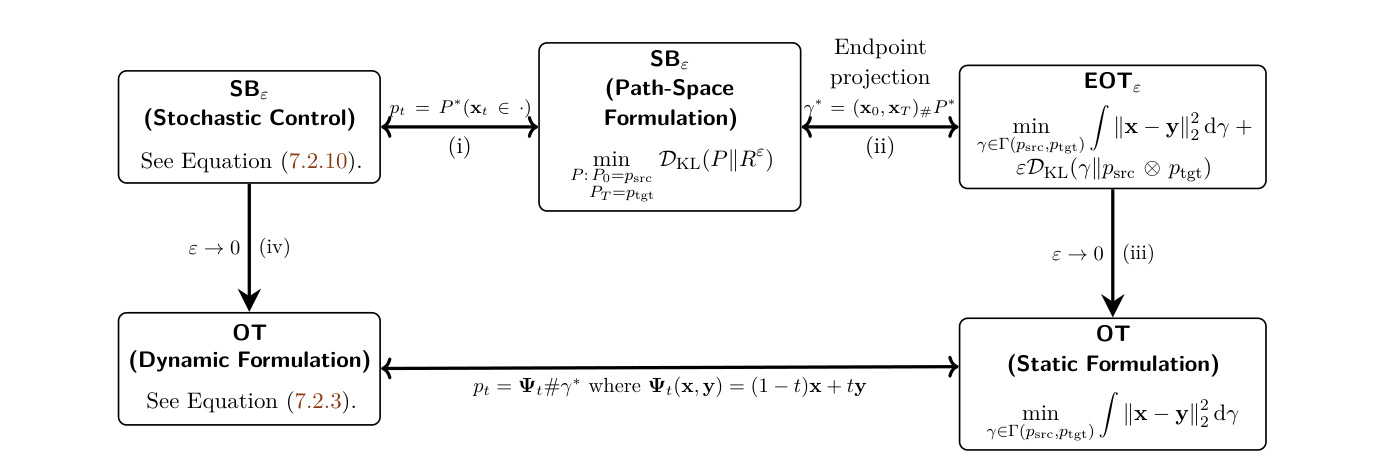
\includegraphics[width=0.95\textwidth,height=0.68\textheight,keepaspectratio]{fig-7-4.jpg}
    \vfill
    \footnotesize
    Source: Created by the authors.\ （論文 Figure~7.4）
\end{frame}
%=============================================
\asmain
\begin{frame}{図7.4 の四つの矢印}
    \begin{enumerate}
        \item[(i)] \textbf{パス空間 SB $\Leftrightarrow$ 確率制御 SB}\\
        同じ橋問題の別表現（§7.2.3）。周辺は $p_t=P^*(\{x_t\in\cdot\})$。
        \item[(ii)] \textbf{ブラウン参照 SB $\Leftrightarrow$ EOT$_\varepsilon$}\\
        最適パスの端点射影 $\gamma^*=(x_0,x_T)_{\#}P^*$ が EOT$_\varepsilon$ を解く。
        \item[(iii)] \textbf{EOT$_\varepsilon\to$ 静的 OT}\\
        $\varepsilon\to 0$ で正則化結合が古典 OT へ。
        \item[(iv)] \textbf{SB$_\varepsilon\to$ 動的 OT}\\
        小さノイズ極限で Benamou--Brenier へ。
    \end{enumerate}
\end{frame}
%=============================================
\asmain
\begin{frame}{(i) パス空間と確率制御}
    パス空間 KL：
    \[
        \mathrm{SB}_\varepsilon(p_{\mathrm{src}},p_{\mathrm{tgt}})
        =
        \min_{P:\,P_0=p_{\mathrm{src}},\,P_T=p_{\mathrm{tgt}}}
        D_{\mathrm{KL}}(P\|R^\varepsilon).
        \tag{7.2.9}
    \]
    ブラウン参照の確率制御形（$T$ 一般）：
    \[
        \min_{v_t}\;
        \frac{1}{2\varepsilon}
        \int_0^T\!\!\int
        \|v_t(x)\|^2\,p_t(x)\,dx\,dt,
        \quad
        dx_t=v_t\,dt+\sqrt{\varepsilon}\,dw_t.
        \tag{7.2.10}
    \]
    \begin{exampleblock}{読み方}
        「参照からどれだけドリフトで歪めるか」のコストが、\\
        パス測度の KL と同じ最適問題を与える。
    \end{exampleblock}
\end{frame}
%=============================================
\asmain
\begin{frame}{(ii)--(iv) を一文で}
    \begin{itemize}
        \item \textbf{(ii)} 端点だけ見れば SB は EOT；\\
        端点を固定したあとの条件付きパスは参照拡散（ブラウン橋など）。
        \item \textbf{(iii)} エントロピーを弱めると、結合は古典 OT へ集中。
        \item \textbf{(iv)} ノイズ $\sqrt{\varepsilon}$ を消すと、制御 SDE は決定的 OT 流へ。
    \end{itemize}
    \begin{alertblock}{静的と動的の底辺}
        静的 OT と動的 OT は、\\
        変位補間 $p_t=\Psi_{t\#}\gamma^*$（$\Psi_t(x,y)=(1-t)x+ty$）で結ばれる。
    \end{alertblock}
\end{frame}
%=============================================
\section{$\varepsilon$ の効果：図7.5}
\asmain
\begin{frame}{図7.5：$\varepsilon$ が大きい／小さいとき}
    \centering
    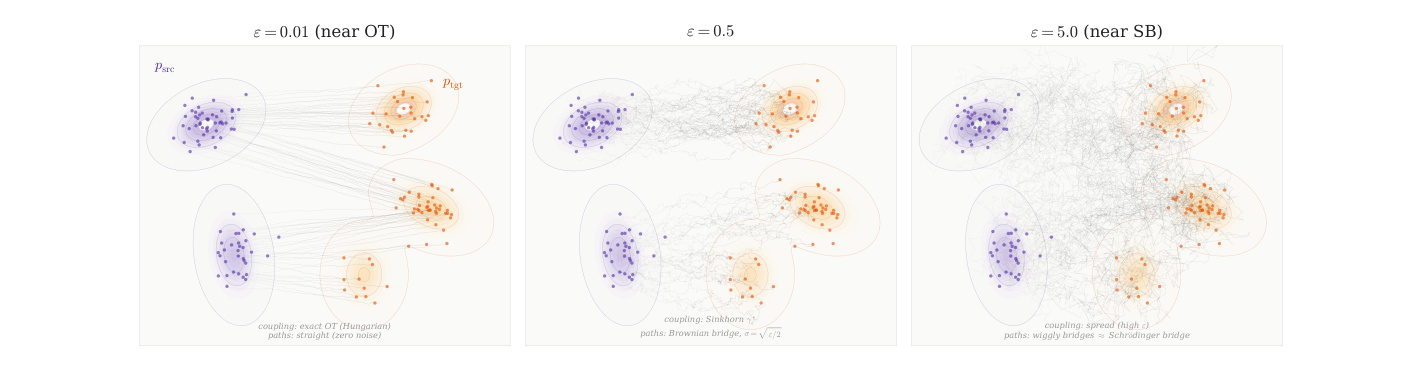
\includegraphics[width=0.98\textwidth,height=0.68\textheight,keepaspectratio]{fig-7-5.jpg}
    \vfill
    \footnotesize
    Source: Created by the authors with AI-assisted coding.\ （論文 Figure~7.5）
\end{frame}
%=============================================
\asmain
\begin{frame}{図7.5 の読み方}
    $\varepsilon$ を大きくすると、\textbf{同時に}二ことが起きる。
    \begin{enumerate}
        \item \textbf{結合 $\gamma_\varepsilon^*$}：遠いターゲットにも質量が広がり、\\
        $\varepsilon\to\infty$ では独立結合 $p_{\mathrm{src}}\otimes p_{\mathrm{tgt}}$ へ。
        \item \textbf{輸送パス}：直線に近く（$\varepsilon$ 小）$\to$ ブラウン橋 $\to$ くねる SB 的橋。
    \end{enumerate}
    \begin{block}{数値の対応}
        左：Hungarian（近似 OT）。中央・右：Sinkhorn。\\
        端点条件付きパスは $\sigma=\sqrt{\varepsilon/2}$ のブラウン橋（Mikami、§7.3.1）。
    \end{block}
\end{frame}
%=============================================
\asmain
\begin{frame}{直感：正則化の強さ}
    \begin{columns}[T,onlytextwidth]
        \begin{column}{0.48\textwidth}
            \begin{block}{$\varepsilon$ 小（near OT）}
                コスト優先。\\
                ほぼ決定的な対応と直線パス。
            \end{block}
        \end{column}
        \begin{column}{0.48\textwidth}
            \begin{block}{$\varepsilon$ 大（near SB）}
                エントロピー／参照らしさ優先。\\
                結合は広がり、パスは確率的。
            \end{block}
        \end{column}
    \end{columns}
    \vfill
    図7.4 の (iii)(iv) は、この連続体の\textbf{左端} $\varepsilon\to 0$ を定理化する。
\end{frame}
%=============================================
\section{7.3.1 SB と EOT の同値}
\asmain
\begin{frame}{区切り：7.3.1 SB と EOT は（双対）同値}
    \tableofcontents[currentsection]
\end{frame}
%=============================================
\asmain
\begin{frame}{7.3.1 のねらい}
    \begin{block}{メッセージ}
        古典 OT が決定的マップを返すのに対し、\\
        SB は\textbf{確率的な粒子流}を返す。ただし端点では EOT と同値。
    \end{block}
    \begin{enumerate}
        \item \textbf{静的}：EOT $\Leftrightarrow$ 静的 Schrödinger（KL to $\widetilde R^\varepsilon$）
        \item \textbf{動的}：二次コスト EOT $\Leftrightarrow$ ブラウン参照 SB（Mikami）
    \end{enumerate}
    どちらからも「端点結合 $\leftrightarrow$ 最適パス測度」の対応が得られる。
\end{frame}
%=============================================
\asmain
\begin{frame}{静的 Schrödinger：参照結合}
    正規化定数
    \[
        Z_\varepsilon
        =
        \iint e^{-c(x,y)/\varepsilon}\,
        p_{\mathrm{src}}(x)\,p_{\mathrm{tgt}}(y)\,dx\,dy
    \]
    のもとで
    \[
        \widetilde R^\varepsilon(x,y)
        :=
        \frac{1}{Z_\varepsilon}\,
        e^{-c(x,y)/\varepsilon}\,
        p_{\mathrm{src}}(x)\,p_{\mathrm{tgt}}(y).
    \]
    \begin{exampleblock}{解釈}
        「コストが低い組ほど大きな重み」を持つ、\\
        独立結合の指数チルト。
    \end{exampleblock}
\end{frame}
%=============================================
\asmain
\begin{frame}{静的同値：式 (7.3.1)}
    任意の $\gamma\in\Gamma(p_{\mathrm{src}},p_{\mathrm{tgt}})$ について
    \[
        \int c\,d\gamma
        +
        \varepsilon D_{\mathrm{KL}}(\gamma\|p_{\mathrm{src}}\otimes p_{\mathrm{tgt}})
        =
        \varepsilon D_{\mathrm{KL}}(\gamma\|\widetilde R^\varepsilon)
        -
        \varepsilon\log Z_\varepsilon.
    \]
    よって（加法定数を除き）
    \[
        \min_{\gamma\in\Gamma}
        \Bigl\{
            \int c\,d\gamma
            +
            \varepsilon D_{\mathrm{KL}}(\gamma\|p_{\mathrm{src}}\otimes p_{\mathrm{tgt}})
        \Bigr\}
        =
        \varepsilon
        \min_{\gamma\in\Gamma}
        D_{\mathrm{KL}}(\gamma\|\widetilde R^\varepsilon)
        -
        \varepsilon\log Z_\varepsilon.
        \tag{7.3.1}
    \]
\end{frame}
%=============================================
\asmain
\begin{frame}{静的同値の帰結}
    EOT$_\varepsilon$ は、制約つき
    \[
        \min_{\gamma\in\Gamma(p_{\mathrm{src}},p_{\mathrm{tgt}})}
        D_{\mathrm{KL}}(\gamma\|\widetilde R^\varepsilon)
    \]
    と\textbf{同じ最小化子}を持つ（値が定数シフトするだけ）。
    \begin{itemize}
        \item 端点結合の最適化 $\Leftrightarrow$ 静的 SB
        \item Sinkhorn が効くのは、この凸なエントロピー問題だから
    \end{itemize}
\end{frame}
%=============================================
\asmain
\begin{frame}{動的同値（ブラウン参照）}
    二次コスト
    \[
        c(x,y)=\frac{\|y-x\|^2}{2T}
    \]
    の EOT は、参照
    \[
        dx_t=\sqrt{\varepsilon}\,dw_t
    \]
    の SB と\textbf{アフィン同値}（値は正スケール＋定数差；最小化子は一致）。
    \begin{block}{端点射影}
        $P^*$：SB 最適パス測度。\\
        $\gamma^*=(x_0,x_T)_{\#}P^*$ は対応する EOT の最適結合。
    \end{block}
\end{frame}
%=============================================
\asmain
\begin{frame}{逆構成：EOT $\to$ SB パス}
    \begin{enumerate}
        \item EOT 最適結合から端点 $(x_0,x_T)\sim\gamma^*$ をサンプリング
        \item 端点条件付きで、参照拡散（ブラウン橋）のパスをサンプリング
        \item $\gamma^*$ で混ぜると最適 SB パス測度 $P^*$ が復元される
    \end{enumerate}
    \begin{exampleblock}{役割分担}
        \textbf{EOT}：どの端点を組むか。\\
        \textbf{参照拡散}：組んだ端点のあいだをどう確率的に運ぶか。
    \end{exampleblock}
\end{frame}
%=============================================
\asmain
\begin{frame}{なぜ二次コストか（ヒューリスティック）}
    パス KL は端点で分解できる。ブラウン遷移はガウスなので
    \[
        -\varepsilon\log p_T(y\mid x)
        =
        \frac{\|y-x\|^2}{2T}
        +
        \mathrm{const}.
    \]
    \begin{alertblock}{要点}
        端点だけの KL が、二次コストの EOT 目的と一致する\\
        （定数差を除く）。これが Mikami 型の同値の核。
    \end{alertblock}
\end{frame}
%=============================================
\assuppl
\begin{frame}{\supplmark：一般参照と端点コスト}
    参照過程の遷移密度を $p_T(y\mid x)$ とすると、端点コストは概ね
    \[
        c(x,y)\;\propto\; -\log p_T(y\mid x)
    \]
    （周辺にしか依らないスケール・加法項を除く）。
    \begin{itemize}
        \item 参照で起きやすい遷移 $\to$ 安いコスト
        \item 起きにくい遷移 $\to$ 高いコスト
    \end{itemize}
    \begin{exampleblock}{SB が EOT より持つ情報}
        端点コストに加え、端点条件付きの\textbf{条件付き確率パス}も参照が決める。
    \end{exampleblock}
\end{frame}
%=============================================
\section{7.3.2 EOT$_\varepsilon\to$ OT}
\asmain
\begin{frame}{区切り：7.3.2 EOT$_\varepsilon$ は $\varepsilon\to 0$ で OT へ}
    \tableofcontents[currentsection]
\end{frame}
%=============================================
\asmain
\begin{frame}{7.3.2 の主張}
    $\gamma_\varepsilon^*$：EOT$_\varepsilon$ の最適計画。\\
    $\gamma^*$：非正則化 OT (7.2.1) の最適計画。
    \begin{block}{標準仮定のもとで}
        $\varepsilon\to 0$ で最適\textbf{値}は OT 値へ収束。\\
        極限計画は OT 最適。OT 最適が唯一なら計画自体も $\gamma^*$ へ。
    \end{block}
    \begin{exampleblock}{実務的意味}
        小さい $\varepsilon$ の EOT（Sinkhorn）を、古典 OT の計算可能な代理にできる。
    \end{exampleblock}
\end{frame}
%=============================================
\asmain
\begin{frame}{定理 7.3.1（非形式）：EOT$_\varepsilon\to$ OT}
    \begin{block}{定理 7.3.1}
        標準仮定のもと
        \[
            \lim_{\varepsilon\to 0}
            \mathrm{EOT}_\varepsilon(p_{\mathrm{src}},p_{\mathrm{tgt}})
            =
            \mathrm{OT}(p_{\mathrm{src}},p_{\mathrm{tgt}}).
        \]
        さらに、極限の最適計画は非正則化 OT の最適結合。\\
        OT 最適が唯一なら、エントロピー最適計画はその最適へ収束する。
    \end{block}
\end{frame}
%=============================================
\assuppl
\begin{frame}{\supplmark：値収束のヒューリスティック（上界）}
    $V_\varepsilon:=\mathrm{EOT}_\varepsilon$、$V_0:=\mathrm{OT}$。\\
    $\gamma^*$ が $D_{\mathrm{KL}}(\gamma^*\|p_{\mathrm{src}}\otimes p_{\mathrm{tgt}})=K<\infty$ なら
    \[
        V_\varepsilon
        \le
        \int c\,d\gamma^*
        +
        \varepsilon K
        =
        V_0+\varepsilon K.
    \]
    よって $\limsup_{\varepsilon\to 0} V_\varepsilon\le V_0$。
\end{frame}
%=============================================
\assuppl
\begin{frame}{\supplmark：値収束のヒューリスティック（下界）}
    KL は非負なので
    \[
        V_\varepsilon
        \ge
        \int c\,d\gamma_\varepsilon^*
        \ge
        V_0
    \]
    （任意計画のコストは $V_0$ 以上）。したがってすべての $\varepsilon>0$ で $V_\varepsilon\ge V_0$、\\
    $\liminf_{\varepsilon\to 0} V_\varepsilon\ge V_0$。
    \begin{alertblock}{合わせると}
        $\lim V_\varepsilon=V_0$。計画の収束にはコンパクト性などが必要\\
        （詳細は Mikami--Thieullen, Peyré--Cuturi など）。
    \end{alertblock}
\end{frame}
%=============================================
\asmain
\begin{frame}{ゼミでの使い方（7.3.2）}
    \begin{itemize}
        \item 図7.5 左端＝「小さい $\varepsilon$ で OT に近い」
        \item Sinkhorn は厳密 OT ソルバではないが、\\
        $\varepsilon\downarrow 0$ で理論的に OT へ近づく代理
        \item コスト $c$ が二次でなくても、同じ極限の議論が使える
    \end{itemize}
\end{frame}
%=============================================
\section{7.3.3 SB$_\varepsilon\to$ OT}
\asmain
\begin{frame}{区切り：7.3.3 SB$_\varepsilon$ は $\varepsilon\to 0$ で OT へ}
    \tableofcontents[currentsection]
\end{frame}
%=============================================
\asmain
\begin{frame}{設定（時間は $T=1$ に正規化）}
    各 $\varepsilon>0$ で、$v_t^\varepsilon$ を SB (7.2.10) の最小化子、\\
    $p_t^\varepsilon$ をその制御 SDE の周辺とする（Fokker--Planck に従う）。
    \[
        dx_t
        =
        v_t^\varepsilon(x_t)\,dt
        +
        \sqrt{\varepsilon}\,dw_t.
    \]
    対して $(p_t^0,v_t^0)$ を Benamou--Brenier OT (7.2.3) の最小化子とする。
\end{frame}
%=============================================
\asmain
\begin{frame}{定理 7.3.2（非形式）：SB$_\varepsilon\to$ OT}
    \begin{block}{定理 7.3.2}
        $\varepsilon\to 0$ で
        \[
            \lim_{\varepsilon\to 0}
            2\varepsilon\,\mathrm{SB}_\varepsilon(p_{\mathrm{src}},p_{\mathrm{tgt}})
            =
            W_2^2(p_{\mathrm{src}},p_{\mathrm{tgt}}),
        \]
        右辺は Benamou--Brenier 形の OT。\\
        適切な仮定のもと、周辺 $p_t^\varepsilon$ と速度 $v_t^\varepsilon$ は部分列で\\
        BB 解 $(p_t^0,v_t^0)$ へ弱収束する（一意ならその解へ）。
    \end{block}
\end{frame}
%=============================================
\asmain
\begin{frame}{なぜ $2\varepsilon$ でスケールするか}
    制御目的 (7.2.10) は概ね
    \[
        \mathrm{SB}_\varepsilon
        \sim
        \frac{1}{2\varepsilon}
        \int_0^1\!\!\int \|v\|^2\,p\,dx\,dt
    \]
    の形。ノイズを消す極限で運動エネルギー
    \[
        \int_0^1\!\!\int \|v\|^2\,p\,dx\,dt
        \;=\;
        W_2^2
    \]
    （BB）に合わせるには、$2\varepsilon\,\mathrm{SB}_\varepsilon$ を見るのが自然。
\end{frame}
%=============================================
\assuppl
\begin{frame}{\supplmark：ヒューリスティック（力学の極限）}
    $\varepsilon\to 0$ でノイズ項が消え、形式的に
    \[
        dx_t=v_t^0(x_t)\,dt
    \]
    （決定的 ODE）。同時に Fokker--Planck
    \[
        \partial_t p_t^\varepsilon
        +
        \nabla\cdot(p_t^\varepsilon v_t^\varepsilon)
        =
        \frac{\varepsilon}{2}\Delta p_t^\varepsilon
    \]
    の拡散項も消え、連続の式
    \[
        \partial_t p_t^0+\nabla\cdot(p_t^0 v_t^0)=0
    \]
    へ。厳密には $\Gamma$-収束などが必要（Léonard 2012, 2014）。
\end{frame}
%=============================================
\asmain
\begin{frame}{実務的な含意（7.3.3）}
    \begin{itemize}
        \item SB$_\varepsilon$ も Sinkhorn 系で解けることが多く、\\
        動的 OT（BB）の微分可能な代理になりうる
        \item 高次元では直接 BB を解くより、\\
        エントロピー／SB 経由の方が現実的な場合がある
        \item 図7.4 の (iv) がこの定理に対応
    \end{itemize}
\end{frame}
%=============================================
\section{まとめ}
\asmain
\begin{frame}{7.3 のまとめ}
    \begin{itemize}
        \item 図7.4：SB（制御／パス）$\leftrightarrow$ EOT $\leftrightarrow$ OT（動的／静的）
        \item 図7.5：$\varepsilon$ 大で結合が広がりパスが確率的；小で OT 的
        \item 7.3.1：静的 KL 同値＋ブラウン参照での動的（Mikami）同値
        \item 7.3.2：EOT$_\varepsilon\to$ 静的 OT（定理 7.3.1）
        \item 7.3.3：スケールした SB$_\varepsilon\to$ 動的 OT / $W_2^2$（定理 7.3.2）
    \end{itemize}
\end{frame}
%=============================================
\asmain
\begin{frame}{次節へ：7.4}
    関係図の上で、拡散モデルを置くとどう見えるか。
    \begin{enumerate}
        \item 拡散 SDE は SB の\textbf{特別な場合}か
        \item それとも half-bridge（片側制約）か
        \item 節タイトルへの答え：いつ Yes / No か
    \end{enumerate}
\end{frame}
